\documentclass[12pt]{report}

% Paquetes LaTeX y estilos globales
\usepackage[utf8]{inputenc}
\usepackage{multicol}
\usepackage{xcolor}
\usepackage{subfigure}
\usepackage[spanish,es-tabla]{babel}
\usepackage[utf8]{inputenc}
\usepackage{graphicx}
\usepackage{titlesec}
\usepackage[bookmarks,breaklinks,colorlinks=true,allcolors=blue]{hyperref}
\usepackage{listings}
\usepackage{inconsolata}
\usepackage{float}
\usepackage{mathpazo} % Fuente Palatino
\usepackage[labelfont=bf]{caption}
\usepackage{comment}

\usepackage[square,numbers]{natbib}
\usepackage[nottoc,notlof,notlot]{tocbibind}  % Mete la bibliografía como capítulo en la TOC, los parámetros excluyen los otros índices de aparecer también
\usepackage{geometry}
\usepackage{amsmath}
\usepackage{parskip}
\usepackage[official]{eurosym}
\usepackage{todonotes}
\usepackage{csquotes}
\usepackage{tocbasic}  % Estilos de la TOC
\usepackage{hyperref}

% Formato del título de capítulos y secciones
\titleformat{\chapter}[block]{\normalfont\huge\bfseries}{\thechapter.}{.5em}{\Huge}[\vspace{2pt}{\titlerule[2pt]}]

\titlespacing*{\chapter}{0pt}{-19pt}{25pt}

\titleformat{\section}[block]{\normalfont\Large\bfseries}{\thesection.}{.5em}{\Large}

\titleformat{\part}[block]{\titlerule[2pt]\normalfont\Huge\bfseries\centering}{Parte \Roman{part}\\\vspace{15pt}}{0pt}{\Huge}[\vspace{2pt}{\titlerule[2pt]}] 

% Tamaños y estilos de elementos en la TOC
\DeclareTOCStyleEntry[
    linefill=\bfseries\TOCLineLeaderFill,
    beforeskip=12pt,
    entrynumberformat=\chapterprefixintoc,
    entryformat=\chaptertocformat,
    pagenumberformat=\chaptertocformat,
    dynnumwidth
]{tocline}{chapter}

\DeclareTOCStyleEntry[
    % linefill=\bfseries\TOCLineLeaderFill,
    beforeskip=30pt,
    entrynumberformat=\chapterprefixintoc,
    entryformat=\parttocformat,
    pagenumberformat=\partpagetocformat,
    numwidth=0pt
]{tocline}{part}

\newcommand\chaptertocformat[1]{\large{\textbf{#1}}}%
\newcommand\chapterprefixintoc[1]{#1}%
\newcommand\parttocformat[1]{\Large{\textbf{#1}}}%
\newcommand\partpagetocformat[1]{} % Don't print the page number for parts

% Alias para estilos de texto comunes
\newcommand{\negritas}[1]{\textbf{#1}}
\newcommand{\cursiva}[1]{\textit{#1}}
\newcommand{\codigo}[1]{\texttt{#1}}

% Formato del código fuente con lstlisting
\lstset{
  basicstyle=\ttfamily,
  breaklines=true,
}

% Márgenes
\geometry{
    a4paper,
    margin=2.75cm
}
\setlength{\marginparwidth}{2cm} 

\pagenumbering{arabic} % Números de página en arábico
 
% Limite de profundidad del índice
\setcounter{tocdepth}{2}

% Eliminar el guionado
\tolerance=1
\emergencystretch=\maxdimen
\hyphenpenalty=10000
\hbadness=10000

% Indentación de párrafos
\setlength{\parindent}{.75cm}

\renewcommand{\lstlistingname}{Extracto de código}
\renewcommand*{\lstlistlistingname}{Índice de extractos de código}

% Comandos para establecer variables
\newcommand{\setTitle}[1]{\def\tfgTitle {#1}}
\newcommand{\setAuthor}[1]{\def\tfgAuthors {#1}}
\newcommand{\setDegree}[1]{\def\tfgDegree {#1}}
\newcommand{\setSupervisor}[1]{\def\tfgSupervisor {#1}}
\newcommand{\setDepartment}[1]{\def\tfgDepartment {#1}}
\newcommand{\setMonth}[1]{\def\tfgMonth {#1}}
\newcommand{\setYear}[1]{\def\tfgYear {#1}}
\newcommand{\setDedication}[1]{\def\tfgDedication {#1}}

% Estilos para el código
% Configuración genérica
\definecolor{codegreen}{rgb}{0,0.6,0}
\definecolor{codegray}{rgb}{0.5,0.5,0.5}
\definecolor{codepurple}{rgb}{0.58,0,0.82}
\definecolor{editorOcher}{rgb}{0.8, 0.3, 0} % #FF7F00 -> rgb(239, 169, 0)
\definecolor{editorGreen}{rgb}{0, 0.5, 0} % #007C00 -> rgb(0, 124, 0)

\lstdefinestyle{listingstyle}{
    backgroundcolor=\color{white},  
    keywordstyle=\bfseries\color{blue},
    numberstyle=\tiny\color{codegray},
    stringstyle=\color{editorGreen},
    commentstyle=\color{codegray},
    basicstyle=\ttfamily\color{black},
    breakatwhitespace=false,         
    breaklines=true,                 
    captionpos=b,                    
    keepspaces=true,                 
    numbers=left,                    
    numbersep=5pt,                  
    showspaces=false,                
    showstringspaces=false,
    showtabs=false,                  
    tabsize=2,
    frame=tb,
    keywords=[2]{True,False},
    literate=%
*{0}{{{\color{editorOcher}0}}}1
{1}{{{\color{editorOcher}1}}}1
{2}{{{\color{editorOcher}2}}}1
{3}{{{\color{editorOcher}3}}}1
{4}{{{\color{editorOcher}4}}}1
{5}{{{\color{editorOcher}5}}}1
{6}{{{\color{editorOcher}6}}}1
{7}{{{\color{editorOcher}7}}}1
{8}{{{\color{editorOcher}8}}}1
{9}{{{\color{editorOcher}9}}}1,
}

\lstset{style=listingstyle}
\lstset{columns=fullflexible}

\lstdefinelanguage{css}{
  keywords={color,background-image:,margin,padding,font,weight,display,position,top,left,right,bottom,list,style,border,size,white,space,min,width, transition:, transform:, transition-property, transition-duration, transition-timing-function},	
  sensitive=true,
  morecomment=[l]{//},
  morecomment=[s]{/*}{*/},
  morestring=[b]',
  morestring=[b]",
  alsoletter={:},
  alsodigit={-}
}
% JavaScript
\lstdefinelanguage{javascript}{
  morekeywords={abstract, arguments, await, boolean, break, byte, case, catch, char, class, const, continue, debugger, default, delete, do, double, else, enum, eval, export, extends, false, final, finally, float, for, function, goto, if, implements, import, in, instanceof, int, interface, let, long, native, new, null, package, private, protected, public, return, short, static, super, switch, synchronized, this, throw, throws, transient, true, try, typeof, var, void, volatile, while, with, yield},
  morecomment=[s]{/*}{*/},
  morecomment=[l]//,
  morestring=[b]",
  morestring=[b]'
}

%Comentarios con todonotes
\newcommand{\Juanmi}[2][]{\todo[inline, color=green!30, caption={ToDo - Juanmi}, #1]{\begin{minipage}{\textwidth-4pt} #2\\ {\bf  -- Juanmi} \end{minipage}}}
\newcommand{\Juanlu}[2][]{\todo[inline, color=gray!20, caption={ToDo - Juanlu}, #1]{\begin{minipage}{\textwidth-4pt} #2 {\bf -- Juanlu}\end{minipage}}}


%%%%%%%%%%%%%%%%%%%%%%%%%%%%%%%%%%%%%%%%%%%%%%%%%%%%%%%%%%%%%%%%%%%%%%%%%%%%%%%%%%%%%

% Variables para la portada
\setTitle{Título del trabajo}
\setAuthor{Nombre del alumno} % Si hay más de un autor, separarlos con \\
\setDegree{Grado en Ingeniería Informática - Ingeniería del Software} % Cambiar si es necesario
\setSupervisor{Nombre del profesor tutor} % Si hay más de un tutor, separarlos con \\
\setDepartment{Lenguajes y Sistemas Informáticos}
\setMonth{junio/julio/diciembre} % Dejar sólo el mes de la convocatoria en que se presenta el trabajo
\setYear{20XX/YY} % Por ejemplo, 2022/23

%%%%%%%%%%%%%%%%%%%%%%%%%%%%%%%%%%%%%%%%%%%%%%%%%%%%%%%%%%%%%%%%%%%%%%%%%%%%%%%%%%%%%

% Dedicatoria del trabajo
% Si no se desea incluir, comentar o borrar la línea siguiente para eliminar la página de dedicatoria
\setDedication{Aquí la dedicatoria del trabajo}

%%%%%%%%%%%%%%%%%%%%%%%%%%%%%%%%%%%%%%%%%%%%%%%%%%%%%%%%%%%%%%%%%%%%%%%%%%%%%%%%%%%%%

% Comienzo del documento
\begin{document}

    % Portada y secciones no numeradas
    \thispagestyle{empty} % Impide que se incluya número de página en la portada
\begin{center}

\vspace*{0.5cm}


\includegraphics[width=\textwidth]{figures/etsiit_ugr_logo.png}

\vspace*{1.5cm}
\begin{large}
TRABAJO FIN DE GRADO
\end{large}

\vspace*{0.1in}
\textbf{\huge \tfgTitle}

\vspace*{.2in}

{\large Realizado por}\\
\textbf{\Large \tfgAuthors}

\vspace*{3cm}

\textbf{Para la obtención del título de}\\
{\large \tfgDegree}

\vspace*{0.2in}

\textbf{Dirigido por}\\
{\large \tfgSupervisor}\\

\vspace*{0.2in}

\textbf{En el departamento de}\\
{\large \tfgDepartment}

\vspace*{.6in}
\textbf{\Large Convocatoria de \tfgMonth, curso \tfgYear}

\end{center}

% Dedicatoria
\ifdefined\tfgDedication
    \newpage
    \thispagestyle{empty}
    
    \vspace*{\fill}
    \begin{center}
    \textit{\tfgDedication}
    \end{center}
    \vspace*{\fill}
\fi

\clearpage\setcounter{page}{1} % Comienza a incluir números de página a partir de aquí
\pagenumbering{roman} % En números romanos
    \chapter*{Agradecimientos}

Este breve, pero sincero, apartado de agradecimientos comienza siendo un homenaje a todas las personas que alguna vez me han ayudado, apoyado o inspirado a lo largo de mi vida. Sin duda, cada uno de ellos ha dejado una huella en mi camino y ha contribuido a que hoy pueda presentar este trabajo.

Quiero expresar mi más profundo agradecimiento a mis padres, quienes siempre han estado a mi lado, brindándome su apoyo incondicional y enseñándome el valor del esfuerzo y la dedicación. Su amor y sacrificio han sido fundamentales en mi formación personal y académica.

A mi hermano, tropezar no significa caer, sino aprender a levantarse. El apoyo y la complicidad que hemos compartido a lo largo de los años han sido una fuente constante de motivación y alegría en mi vida. Gracias por todo.

A mis amigos, cada uno con sus propias historias, vivencias y enseñanzas, cada uno entrelazando su camino con el mío en épocas y distancias diferentes. Gracias por estar siempre a mi lado, por hacer que el viaje sea más llevadero y por compartir momentos inolvidables.

A mi novia, Laura, por su amor, paciencia y comprensión. Tu apoyo constante ha sido mi mayor motivación en cada paso que doy, tu presencia ilumina mis días y me impulsa a seguir adelante, incluso en los momentos más difíciles.

En último lugar, pero no menos importante, quiero agradecer a mi director de TFG, Juan Luis Jiménez Laredo, por su orientación, motivación, esfuerzo y dedicación durante todo el proceso. Su experiencia y conocimientos han sido invaluables para el desarrollo de este trabajo, y su apoyo constante me ha permitido superar los desafíos que se presentaron en el camino. Te has convertido sin duda en una fuente de inspiración y un modelo a seguir en mi vida académica y profesional. Gracias por tu confianza en mí y por guiarme en este proceso.

A todos ellos, mi más sincero agradecimiento. Este trabajo es un reflejo de su apoyo y confianza en mí, y espero que sea un digno homenaje a todo lo que han hecho por mí. Gracias por ser parte de mi vida y por ayudarme a alcanzar mis metas.
    \newpage
\begin{center}
    {\large \textbf{TempusUGR - Desarrollo de una Aplicación de Gestión de Horarios Universitarios Basada en Microservicios Interoperable con Servicios de Calendario Externos}}
    
    \vspace{0.3cm}
    {\normalsize Juan Miguel Acosta Ortega} 
    
    \vspace{0.3cm}
\end{center}

\vspace{0.5cm}

\textbf{Palabras clave:} Microservicios, Contenerización, Calendario Académico, Interoperabilidad, Backend, Autenticación

\vspace{0.5cm}

\textbf{Resumen:}

El presente Trabajo Fin de Grado aborda el diseño e implementación de un sistema backend para la gestión centralizada y la distribución dinámica del calendario académico de la Universidad de Granada. El proyecto nace de la necesidad de modernizar el acceso a la información académica, superando los desafíos de la dispersión de datos y la falta de integración con las herramientas de productividad digital actuales.

La solución se fundamenta en una arquitectura de microservicios contenerizados, seleccionada por su alta escalabilidad, resiliencia y facilidad de mantenimiento. El núcleo del sistema es una plataforma de suscripción que permite a estudiantes y profesores, previa autenticación segura con sus credenciales universitarias, generar calendarios personalizados. Cada usuario puede seleccionar los grupos de teoría y prácticas correspondientes a su matrícula o docencia, obteniendo una vista unificada y detallada que incluye asignaturas, aulas y profesorado.

Un pilar fundamental del proyecto es la interoperabilidad con servicios de calendario externos. El sistema permite a los usuarios exportar y sincronizar sus horarios personalizados con plataformas de amplio uso como Google Calendar. Esta funcionalidad garantiza el acceso a la información académica en tiempo real y desde cualquier dispositivo, eliminando la necesidad de consultas manuales y propensas a errores.

En definitiva, este trabajo no solo desarrolla una aplicación funcional, sino que establece una infraestructura tecnológica que optimiza la gestión del tiempo y mejora significativamente la experiencia de usuario para toda la comunidad de la UGR, promoviendo una gestión académica más eficiente, accesible y centralizada.

    \chapter*{Abstract}
This Final Degree Project addresses the design and implementation of a backend system for the centralized management and dynamic distribution of the academic calendar of the University of Granada (UGR). The project stems from the need to modernize access to academic information, overcoming the challenges of data dispersion and the lack of integration with current digital productivity tools.

The proposed solution is based on a containerized microservices architecture, selected for its high scalability, resilience, and ease of maintenance. The core of the system is a subscription platform that allows students and faculty, after secure authentication with their university credentials, to generate personalized calendars. Each user can select the lecture and practical groups corresponding to their enrollment or teaching assignments, obtaining a unified and detailed view that includes subjects, classrooms, and instructors.

A fundamental pillar of the project is interoperability with external calendar services. The system enables users to export and synchronize their personalized schedules with widely used platforms such as Google Calendar. This functionality ensures access to academic information in real-time and from any device, eliminating the need for manual and error-prone lookups.

In conclusion, this project not only develops a functional application but also establishes a technological infrastructure that optimizes time management and significantly enhances the user experience for the entire UGR community, promoting a more efficient, accessible, and centralized academic management.

\vspace{.5cm}

\textbf{Keywords:} Microservices, Containerization, Academic Calendar, Interoperability, Backend, Authentication
    
    % Índice del documento y de figuras
    \begingroup
        % Los enlaces son normalmente azules, pero en los índices se configuran a negro para que no aparezca todo azul
        \hypersetup{linkcolor=black}
        \tableofcontents
        \listoffigures
        \listoftables
        \lstlistoflistings
    \endgroup
    
    % Cambia el estilo de números de página de romanos a normal
    \clearpage\pagenumbering{arabic}
    
    % Capítulos del trabajo
    \chapter{Ejemplos de uso de LaTeX}\label{cap:ejemplos}

\todo[inline]{Este capítulo se incluye únicamente como ayuda y referencia de uso de \LaTeX. No debe aparecer en el documento final.}

\section{Introducción}
En este capítulo se muestran ejemplos de uso de \LaTeX{} para operaciones comunes. 

\section{Estilos}\label{sec:estilos}
Se pueden aplicar estilos al texto como \textbf{negritas}, \textit{cursiva}, \underline{subrayado} y \texttt{monoespaciado}. También se \textcolor{red}{pueden} \textcolor{blue}{aplicar} \textcolor{green}{colores}, y \underline{\textit{combinar}} \textbf{\textcolor{red}{estilos}}. Se recomienda usar sólo negritas para hacer énfasis, y no abusar de este recurso.

Por comodidad para usuarios no habituados con LaTeX, esta plantilla define algunos alias de comandos más fáciles de recordar para estilos de texto comunes: \negritas{negritas}, \cursiva{cursiva} y \codigo{código}.

\section{Listados}
Con itemize se pueden crear listas no numeradas:

\begin{itemize}
    \item Fresas
    \item Melocotones
    \item Piñas
    \item Nectarinas
\end{itemize}

De manera similar, enumerate permite crear listas numeradas:

\begin{enumerate}
    \item Elaborar la memoria del TFG
    \item Elaborar la presentación
    \item Presentar el TFG
    \item Solicitar el título de Grado
\end{enumerate}

\section{Subsecciones}
Se pueden definir subsecciones con el comando \texttt{subsection}:

\subsection{Primera subsección}\label{sec:subseccion}
Esto es una subsección

\subsection{Segunda subsección}
Esto es otra subsección.

\subsubsection{Sub-sub-sección}
Este es un tercer nivel de profundidad, que no aparece en el índice general. Se recomienda no utilizarlo, si es posible.

\section{Imágenes y figuras}
Todas las imágenes y figuras del documento se incluirán en la carpeta ``figures''. Se pueden incluir de la siguiente manera:

\begin{figure}[htp]
    \centering
    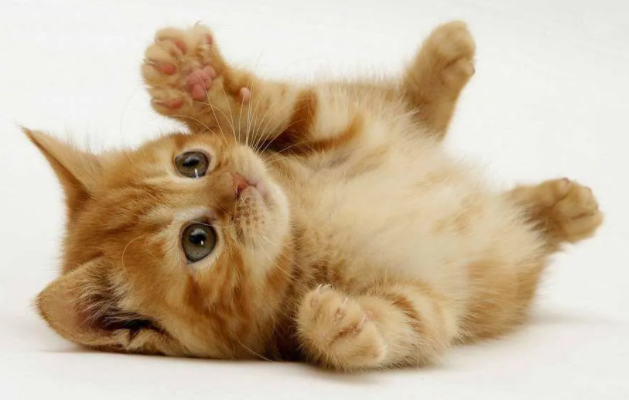
\includegraphics[width=0.7\textwidth]{figures/ejemplo.png}
    \caption{Un feroz depredador}
    \label{fig:ejemplo}
\end{figure}

Observe que las figuras se numeran automáticamente según el capítulo y el número de figuras que hayan aparecido anteriormente en dicho capítulo. Existen muchas maneras de definir el tamaño de una figura, pero se aconseja utilizar la mostrada en este ejemplo: se define el ancho de la figura como un porcentaje del ancho total de la página, y la altura se escala automáticamente. De esta manera, el ancho máximo de una figura sería 1.0 * textwidth, lo que aseguraría que se muestra al máximo tamaño posible sin sobrepasar los márgenes del documento.

Tenga en cuenta que LaTeX intenta incluir las figuras en el mismo sitio donde se declaran, pero en ocasiones no es posible por motivos de espacio. En esos casos, LaTeX colocará la figura lo más cerca posible de su declaración, puede que en una página diferente. Esto es un comportamiento normal.

\section{Tablas}
Existe una gran variedad de formas de crear tablas en LaTeX puro, y todas ellas tienen cierta complejidad. A continuación se muestra un ejemplo simple de tabla nativa, en la Tabla \ref{table:ejemplo}. Se recomienda crear un archivo en la carpeta \textit{tables} por cada tabla nativa que se desee incluir, y enlazarla mediante el comando \texttt{input}.

\begin{table}[htp]
\centering

    % Esta primera línea define las columnas de la tabla. Los posibles tipos de columna son:
    % c: texto centrado
    % l: texto alineado a la izquierda
    % r: texto centrado a la derecha
    % p: columna de ancho fijo
    % Las columnas tienen ancho dinámico según la anchura máxima de los elementos que contengan.

    % Las columnas l/r/c no parten el texto en filas diferentes si éste es demasiado largo. Para ello, puede utilizar el tipo de columna de ancho fijo "p".
    
    % Las barras verticales | se usan para definir los bordes verticales de la tabla. Pruebe a eliminar algunas y observe qué ocurre.
    \begin{tabular}{ | l | c | r | p{2cm} | }
        
        % A continuación van las filas de la tabla. En cada fila, las columnas se separan con el carácter &
        % Para terminar una fila se usa \\
        % Para incluir un borde horizontal entre filas se usa \hline

        % Cabecera con textos en negrita:
        \hline
        \textbf{Columna L} & \textbf{Columna C} & \textbf{Columna R} & \textbf{Columna P}\\
        \hline
        
        % Cuerpo de la tabla:
        Texto de ejemplo & Texto de ejemplo & Texto de ejemplo & Texto de ejemplo\\
        \hline
        ABC & DEF & HIJ & KLM\\
        \hline
        
    \end{tabular} 
    
    \caption{Tabla LaTeX de ejemplo}
    \label{table:ejemplo} 
\end{table}


Para tablas con un formato más complejo, considere la posibilidad de diseñarla usando otro software externo (por ejemplo Excel) e incluirla de manera similar a una figura. \textbf{Observe en el código LaTeX a continuación cómo usar el comando \texttt{captionof\{table\}}, en lugar de simplemente \texttt{caption}, hace que se liste como una Tabla en lugar de como una Figura}:

\begin{figure}[htp]
    \centering
    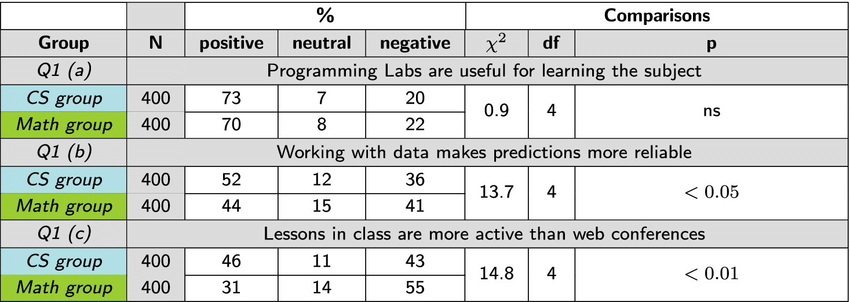
\includegraphics[width=1.0\textwidth]{tables/complex_table.png}
    \captionof{table}{Tabla compleja introducida como figura}
    \label{table:ejemplo2}
\end{figure}

\section{Referencias}
Observe cómo en el código fuente de esta sección se ha usado varias veces el comando \texttt{label}. Este comando permite marcar un elemento, ya sea capítulo, sección, figura, etc. para hacer una referencia numérica al mismo. Para referenciar una label se usa el comando \texttt{ref} incluyendo el nombre de la referencia:

Este es el capítulo \ref{cap:ejemplos}.

En la sección \ref{sec:estilos} se muestran ejemplos de estilos.

La subsección \ref{sec:subseccion} explica...

En la Figura \ref{fig:ejemplo} vemos que...

Esto evita que tengamos que escribir directamente los índices de las secciones y figuras que queremos mencionar, ya que LaTeX lo hace por nosotros y además se encarga de mantenerlos actualizados en caso de que cambien (pruebe a mover este capítulo al final del documento y observe cómo se actualizan automáticamente todos los índices referenciados). Además, las referencias mediante ``ref'' actúan como hipervínculos dentro del documento que llevan al elemento referenciado al pulsar en ellas.

Es habitual nombrar las ``label'' con un prefijo que indica el tipo de elemento para encontrarlo luego más fácilmente, pero no es obligatorio.

\section{Extractos de código}

Se pueden incluir extractos de código mediante lstlisting:

\begin{lstlisting}[language=Python, caption={Código Python}, label={cod:python}, captionpos=b]
num = float(input("Enter a number: "))
if num > 0:
   print("Positive number")
elif num == 0:
   print("Zero")
else:
   print("Negative number")
\end{lstlisting}

Para evitar tener que incluir el código directamente en el texto del documento, se pueden guardar en archivos separados y referenciarlos:

\lstinputlisting[
    float,
    floatplacement=!htp,
    language=Java,
    label=cod:java,
    caption=Código Java
]{code/java_example.java}

\lstinputlisting[
    float,
    floatplacement=!htp,
    language=html,
    label=cod:html,
    caption=Código HTML
]{code/html_example.html}

\lstinputlisting[
    float,
    floatplacement=!htp,
    language=javascript,
    label=cod:js,
    caption=Código JavaScript
]{code/javascript_example.js}

Los extractos de código también se pueden referenciar mediante label/ref: Extractos de código \ref{cod:python}, \ref{cod:java}, \ref{cod:html}, \ref{cod:js}. 

\section{Enlaces}
Puede enlazar una web externa mediante el comando \texttt{url}: \url{https://www.example.com}. También se puede vincular un enlace a un texto mediante el comando href: \href{https://www.example.com}{dominio de ejemplo}.

\section{Citas y bibliografía}
En LaTeX, los elementos de la bibliografía se almacenan en un fichero bibliográfico en un formato llamado BibTeX, en el caso de este proyecto se encuentran en ``bibliografia.bib''. Para citar un elemento se usa el comando \texttt{cite}. Se pueden citar tanto artículos científicos \cite{borrego2019} como enlaces web \cite{webETSII}. 

También se puede usar el comando \texttt{citet} para incluir una referencia junto con el nombre de su autor o autores: \citet{borrego2021}. Todas las citas se numeran automáticamente y se incluyen en la sección de bibliografía del trabajo. El orden por defecto es según su orden de aparición en el documento. Para ordenarlas por orden alfabético del autor, puede modificar el comando \texttt{bibliographystyle} del archivo principal y reemplazar su valor por el estilo \texttt{plainnat} (orden alfabético, nombres completos) o \texttt{abbrvnat} (orden alfabético, nombres abreviados).

Observe cómo los elementos bibliográficos almacenados en ``bibliografia.bib'' tienen una etiqueta asociada, que es la que se usa al citarlos mediante cite. \textbf{Añadir una referencia al fichero bibliográfico no hace que ésta aparezca automáticamente en la sección de bibliografía del trabajo, es necesario citarla en algún lugar del mismo}.

\section{Ecuaciones}
LaTeX tiene un potente motor para mostrar ecuaciones matemáticas y un amplio catálogo de símbolos matemáticos. El entorno matemático se puede activar de muchas maneras. Para incluir ecuaciones simples en un texto se pueden rodear de símbolos dólar: $1 + 2 = 3$, $\sqrt{81} = 3^2 = 9$, $\forall x \in y~\exists~z : S_z < 4$.

Las ecuaciones más complejas pueden expresarse aparte y son numeradas: ecuación \ref{eq:ecuacion}.

\begin{equation}\label{eq:ecuacion}
\lim_{x\to 0}{\frac{e^x-1}{2x}}
 \overset{\left[\frac{0}{0}\right]}{\underset{\mathrm{H}}{=}}
 \lim_{x\to 0}{\frac{e^x}{2}}={\frac{1}{2}}
 +7 \int_0^2
  \left(
    -\frac{1}{4}\left(e^{-4t_1}+e^{4t_1-8}\right)
  \right)\,dt_1
\end{equation}

Dispone \href{http://www.yann-ollivier.org/latex/texsymbols.pdf}{aquí} de un amplio listado de símbolos que pueden usarse en modo matemático.

\section{Caracteres y símbolos especiales}
Algunos caracteres y símbolos deben ser escapados para poder representarse en el documento, ya que tienen un significado especial en LaTeX. Algunos de ellos son:

\begin{itemize}
    \item El símbolo dólar \$ se usa para ecuaciones.
    \item El tanto por ciento \% se usa para comentarios en el código fuente.
    \item El símbolo euro \euro{} suele dar problemas si se escribe directamente.
    \item El guión bajo \_ se usa para subíndices en modo matemático.
    \item Las comillas deben expresarse `así' para comillas simples y ``así'' para comillas dobles. Las comillas españolas pueden expresarse \textquote{así}.
    \item La barra invertida o contrabarra \textbackslash{} se usa para comandos LaTeX.
    \item Otros símbolos que deben escaparse son las llaves \{ \}, el ampersand \&, la almohadilla \# y los símbolos mayor que \textgreater{} y menor que \textless{}.
\end{itemize}
    \chapter{Introducción}\label{cap:introduccion}

\section{Motivación}

La arquitectura de microservicios ha emergido como un paradigma fundamental en el desarrollo de sistemas complejos y escalables. Su enfoque modular y distribuido ofrece ventajas claras en términos de flexibilidad, mantenibilidad y despliegue independiente. Sin embargo, la implementación exitosa de una arquitectura de microservicios conlleva una serie de desafíos técnicos que resultan atractivos desde una perspectiva de aprendizaje y desarrollo profesional.

Este proyecto de fin de grado se presenta como una oportunidad perfecta para explorar de manera profunda los entresijos de esta arquitectura. Conceptos como la comunicación eficiente entre servicios (síncrona y asíncrona), la implementación de un API Gateway robusto para la gestión centralizada de peticiones, enrutamiento, seguridad ... , la aplicación de mecanismos de seguridad en un entorno distribuido, y las estrategias de balanceo de carga para garantizar la disponibilidad del sistema, representan áreas de gran interés práctico y teórico.

El desarrollo de un sistema de calendario personalizado para la Universidad de Granada, basado en una arquitectura de microservicios, permitirá no solo consolidar conocimientos teóricos, sino también enfrentarse a los retos inherentes a la construcción de un sistema distribuido real. La necesidad de diseñar APIs claras y bien definidas, gestionar la persistencia de datos en múltiples servicios, asegurar la consistencia y la tolerancia a fallos, y monitorizar el rendimiento del sistema en su conjunto, proporcionarán una experiencia de aprendizaje invaluable. En definitiva, este proyecto se concibe como un vehículo para comprender y aplicar de manera práctica los principios y las mejores prácticas asociadas a la arquitectura de microservicios, un campo con una alta demanda en la industria del desarrollo de software.

\section{Estructura de la memoria}

La estructura de la memoria se divide en los siguientes capítulos:

\begin{itemize}
    \item \textbf{Capítulo 1: Introducción.} En este capítulo se presenta la motivación del trabajo y la estructura de la memoria.
    \item \textbf{Capítulo 2: Descripción del problema.} En este capítulo se describe el problema que se va a resolver en el trabajo.
    \item \textbf{Capítulo 3: Estado del arte.} En este capítulo se presenta un resumen del estado del arte tanto en el ámbito de sistemas de gestión de horarios como en el ámbito de sistemas de información basados en web.
    \item \textbf{Capítulo 4: Especificación de requisitos.} En este capítulo se presentan las personas, escenarios, y los requisitos del sistema en forma de historias de usuario y requisitos funcionales, no funcionales, y de información.
    \item \textbf{Capítulo 5: Planificación.} En este capítulo se presenta la planificación temporal de trabajo, la metodología de desarrollo escogida y su implementación. Además se presenta un presupuesto del trabajo.
    \item \textbf{Capítulo 6: Diseño.} En este capítulo se presenta el diseño de la arquitectura de microservicios, de la API REST Implementada, de las bases de datos y del frontend desarrollado.
    \item \textbf{Capítulo 7: Implementación.} En este capítulo se presenta la implementación del sistema dividido en los sprints realizados.
    \item \textbf{Capítulo 8: Despliegue.} En este capítulo se presenta el despliegue del sistema en el servidor de la UGR con lo que todo ello conlleva ( gestión del servidor, SSL, HTTPS, dominio, etc.).
    \item \textbf{Capítulo 9: Conclusiones.} En este capítulo se presentan las conclusiones y trabajos futuros planteados.
    \item \textbf{Anexo A: Glosario.} En este anexo se presenta un glosario con las definiciones de términos técnicos utilizados a lo largo del trabajo.
\end{itemize}
    \chapter{Estudio previo}\label{cap:planificación}

\section{Introducción}
Breve introducción al capítulo

\section{Objetivos}

\section{Metodología}

\section{Planificación}

\section{Presupuesto}

\section{Conclusiones}
    \chapter{Análisis del problema}\label{cap:analisis}

\section{Introducción}
En este capítulo explicaremos...

\section{Requisitos de información}
Los requisitos de información son...

\section{Requisitos funcionales}
Los requisitos funcionales son...

\section{Requisitos no funcionales}
Los requisitos no funcionales son...

\section{Conclusiones}
En este capítulo concluimos que...
    \input{sections/04_Diseño}
    \chapter{Implementación}\label{cap:implementacion}

\section{Introducción}
En este capítulo explicaremos...

\section {Herramientas}

\section{Conclusiones}
En este capítulo concluimos que...
    \chapter{Pruebas}\label{cap:pruebas}

\section{Introducción}
En este capítulo explicaremos...

\section{Conclusiones}
En este capítulo concluimos que...
    \chapter{Conclusiones}\label{cap:conclusiones}



    % Bibliografía
    \bibliographystyle{unsrtnat}
    \bibliography{bibliografia.bib}
        

% Fin del documento
\end{document}
